% Options for packages loaded elsewhere
\PassOptionsToPackage{unicode}{hyperref}
\PassOptionsToPackage{hyphens}{url}
\PassOptionsToPackage{dvipsnames,svgnames,x11names}{xcolor}
%
\documentclass[
  11pt,
  letterpaper,
]{article}
\usepackage{amsmath,amssymb}
\usepackage{iftex}
\ifPDFTeX
  \usepackage[T1]{fontenc}
  \usepackage[utf8]{inputenc}
  \usepackage{textcomp} % provide euro and other symbols
\else % if luatex or xetex
  \usepackage{unicode-math} % this also loads fontspec
  \defaultfontfeatures{Scale=MatchLowercase}
  \defaultfontfeatures[\rmfamily]{Ligatures=TeX,Scale=1}
\fi
\usepackage{lmodern}
\ifPDFTeX\else
  % xetex/luatex font selection
\fi
% Use upquote if available, for straight quotes in verbatim environments
\IfFileExists{upquote.sty}{\usepackage{upquote}}{}
\IfFileExists{microtype.sty}{% use microtype if available
  \usepackage[]{microtype}
  \UseMicrotypeSet[protrusion]{basicmath} % disable protrusion for tt fonts
}{}
\makeatletter
\@ifundefined{KOMAClassName}{% if non-KOMA class
  \IfFileExists{parskip.sty}{%
    \usepackage{parskip}
  }{% else
    \setlength{\parindent}{0pt}
    \setlength{\parskip}{6pt plus 2pt minus 1pt}}
}{% if KOMA class
  \KOMAoptions{parskip=half}}
\makeatother
\usepackage{xcolor}
\usepackage[margin=1in]{geometry}
\usepackage{graphicx}
\makeatletter
\def\maxwidth{\ifdim\Gin@nat@width>\linewidth\linewidth\else\Gin@nat@width\fi}
\def\maxheight{\ifdim\Gin@nat@height>\textheight\textheight\else\Gin@nat@height\fi}
\makeatother
% Scale images if necessary, so that they will not overflow the page
% margins by default, and it is still possible to overwrite the defaults
% using explicit options in \includegraphics[width, height, ...]{}
\setkeys{Gin}{width=\maxwidth,height=\maxheight,keepaspectratio}
% Set default figure placement to htbp
\makeatletter
\def\fps@figure{htbp}
\makeatother
\setlength{\emergencystretch}{3em} % prevent overfull lines
\providecommand{\tightlist}{%
  \setlength{\itemsep}{0pt}\setlength{\parskip}{0pt}}
\setcounter{secnumdepth}{-\maxdimen} % remove section numbering
% definitions for citeproc citations
\NewDocumentCommand\citeproctext{}{}
\NewDocumentCommand\citeproc{mm}{%
  \begingroup\def\citeproctext{#2}\cite{#1}\endgroup}
\makeatletter
 % allow citations to break across lines
 \let\@cite@ofmt\@firstofone
 % avoid brackets around text for \cite:
 \def\@biblabel#1{}
 \def\@cite#1#2{{#1\if@tempswa , #2\fi}}
\makeatother
\newlength{\cslhangindent}
\setlength{\cslhangindent}{1.5em}
\newlength{\csllabelwidth}
\setlength{\csllabelwidth}{3em}
\newenvironment{CSLReferences}[2] % #1 hanging-indent, #2 entry-spacing
 {\begin{list}{}{%
  \setlength{\itemindent}{0pt}
  \setlength{\leftmargin}{0pt}
  \setlength{\parsep}{0pt}
  % turn on hanging indent if param 1 is 1
  \ifodd #1
   \setlength{\leftmargin}{\cslhangindent}
   \setlength{\itemindent}{-1\cslhangindent}
  \fi
  % set entry spacing
  \setlength{\itemsep}{#2\baselineskip}}}
 {\end{list}}
\usepackage{calc}
\newcommand{\CSLBlock}[1]{\hfill\break\parbox[t]{\linewidth}{\strut\ignorespaces#1\strut}}
\newcommand{\CSLLeftMargin}[1]{\parbox[t]{\csllabelwidth}{\strut#1\strut}}
\newcommand{\CSLRightInline}[1]{\parbox[t]{\linewidth - \csllabelwidth}{\strut#1\strut}}
\newcommand{\CSLIndent}[1]{\hspace{\cslhangindent}#1}
\ifLuaTeX
  \usepackage{selnolig}  % disable illegal ligatures
\fi
\usepackage{bookmark}
\IfFileExists{xurl.sty}{\usepackage{xurl}}{} % add URL line breaks if available
\urlstyle{same}
\hypersetup{
  pdftitle={Perspectives on Quantum Technologies in Mexican Digital Transformation},
  pdfauthor={Edgar Valdés, Hadox Research Labs},
  colorlinks=true,
  linkcolor={blue},
  filecolor={blue},
  citecolor={blue},
  urlcolor={blue},
  pdfcreator={LaTeX via pandoc}}

\title{Perspectives on Quantum Technologies in Mexican Digital
Transformation\thanks{Prepared for the Quantum Technologies track of the
twenty-third edition of the Global Information Technology Management
Association Annual Conference, Monterrey, Mexico, May 6-8, 2026, for
which Edgar Antonio Valdés Porras serves as Track Chair. The author
gratefully acknowledges Rogelio Marín and the Centro de Investigación en
Matemáticas, A.C. for intellectual support and institutional context.
All interpretations and remaining errors are the author's
responsibility.}}
\author{Edgar Valdés, Hadox Research Labs}
\date{April 2026}

\begin{document}
\maketitle

\section{Abstract}\label{abstract}

Quantum technologies are examined as an emerging layer of Mexican
digital transformation. Rather than treating quantum computing as a
distant replacement for existing digital policy, the analysis situates
quantum technologies within a strategic infrastructure agenda that
intersects with cybersecurity, measurement, cloud access,
high-performance computing, artificial intelligence, industrial
modernization, and scientific sovereignty. The evidentiary base includes
enterprise-adoption research, OECD data on business readiness and
national quantum strategies, NIST/NSA/CISA cybersecurity guidance,
OpenAlex bibliometric indicators, and recent studies on hybrid HPC-QC
workflows. The evidence indicates that quantum adoption is constrained
less by awareness than by organizational readiness, technical talent,
validated use cases, standards, procurement discipline, and absorptive
capacity. Mexico's relevant near-term problem is therefore not immediate
ownership of universal fault-tolerant quantum hardware, but the
construction of capabilities in post-quantum cryptography, quantum
sensing, HPC-QC workflow experimentation, quantum software, metrology,
standards, and frontier research. OpenAlex data identify a small but
measurable Mexican research base in quantum technology, led in the
extracted dataset by UNAM, IPN, and Tecnologico de Monterrey. Mexico's
quantum transition is consequently framed as a sequenced national
capability problem: cryptographic migration and sensing pilots first,
cloud-mediated and HPC-mediated experimentation and workforce formation
second, and selective frontier research and international integration as
the long-term platform for technological autonomy.

\textbf{Keywords:} Mexico, digital transformation, quantum technologies,
post-quantum cryptography, quantum sensing, quantum computing,
high-performance computing, HPC-QC integration, innovation policy,
technological sovereignty

\section{1. Introduction}\label{introduction}

The literature and policy discourse on Mexican digital transformation
have generally emphasized artificial intelligence, machine learning,
cloud infrastructure, distributed ledgers, open data, automation, and
digital government. These technologies remain central to the
modernization of public administration, finance, health, logistics,
manufacturing, and urban services. They do not, however, exhaust the
technological horizon of the coming decade. Quantum technologies
introduce a different layer of digital transformation: one concerned not
only with data processing, but also with the physical limits of
computation, measurement, security, synchronization, simulation, and
communication.

The analysis examines how quantum technologies can be framed within the
Mexican digital transformation agenda. It does not assume that Mexico
will reproduce the quantum strategies of the United States, China, the
European Union, or the United Kingdom. Rather, it asks how a
middle-income, manufacturing-intensive, digitally uneven, scientifically
capable country can participate in the quantum transition through
selective capability building. The central proposition is that Mexico's
first-order quantum policy problem is not hardware sovereignty in
universal quantum computing, but readiness: the ability to understand,
procure, regulate, test, and integrate quantum technologies as they
become relevant to national problems.

Four research questions structure the article. First, what does the
international evidence on quantum adoption suggest about organizational
and national readiness? Second, what quantitative indicators can be used
to approximate Mexico's current absorptive capacity in quantum
technologies? Third, which domains of quantum technology are most
relevant to Mexican digital transformation in the 2025-2035 horizon?
Fourth, how can Mexican HPC infrastructure mediate the transition from
classical scientific computing to quantum computing?

\section{2. Literature and Policy
Background}\label{literature-and-policy-background}

Quantum technologies are commonly organized into four domains: quantum
computing, quantum sensing, quantum communication, and post-quantum
cryptography. These domains differ in technological maturity,
infrastructure requirements, commercial pathways, and relevance to
national policy. Quantum computing remains the most visible domain, but
its broad economic impact depends on fault-tolerant architectures,
logical qubits, algorithms, and cloud-mediated experimentation
(\citeproc{ref-preskill2018}{Preskill 2018};
\citeproc{ref-bova2020}{Bova, Goldfarb, and Melko 2020}). Quantum
sensing is closer to deployment in selected applications because it uses
quantum effects to improve measurement rather than to perform universal
computation. Quantum communication provides specialized security
primitives and long-term network possibilities, but it faces cost,
distance, and device-assurance challenges. Post-quantum cryptography is
a software and standards transition that can be pursued before
cryptographically relevant quantum computers exist.

The quantum computing pathway is also an HPC pathway. Recent studies on
hybrid quantum-classical workflows frame quantum processing units as
accelerators embedded in scientific computing environments rather than
as stand-alone replacements for supercomputers
(\citeproc{ref-cranganore2024}{Cranganore et al. 2024};
\citeproc{ref-beck2024}{Beck et al. 2024}; \citeproc{ref-liu2024}{Liu et
al. 2024}). For Mexico, QCaaS and domestic HPC capacity are
complementary: cloud-based QPUs can support experimentation, while HPC
centers provide simulation, benchmarking, data preparation, workflow
integration, error-mitigation loops, and validation against classical
baselines.

The adoption literature indicates that quantum readiness is not a simple
function of technological availability. Kwon et al.
(\citeproc{ref-kwon2026}{2026}) analyze enterprise intention to adopt
quantum computing through a sequential explanatory design based on
expert interviews and a survey of 250 IT decision-makers. They find that
adoption intention is shaped by perceived quantum advantage, belief in
quantum superiority, budget continuity, regulatory support,
organizational resistance, financial risk, and co-creation. This
evidence is important for Mexico because it suggests that adoption
depends on institutional conditions and absorptive capacity, not only on
hardware maturity.

The theoretical framing follows the literature on absorptive capacity
and national innovation systems. Absorptive capacity describes the
ability to recognize, assimilate, and use external knowledge
(\citeproc{ref-cohen1990}{Cohen and Levinthal 1990}). National
innovation systems locate technological performance in networks of
firms, universities, public agencies, standards bodies, and financial
institutions rather than in isolated inventions
(\citeproc{ref-lundvall1992}{Lundvall 1992};
\citeproc{ref-nelson1993}{Nelson 1993}). This matters for quantum policy
because scientific capability alone does not create adoption. Adoption
requires complementary assets: standards, procurement competence,
cybersecurity governance, technical education, cloud access,
laboratories, and sectoral demand.

OECD readiness data reinforce this conclusion. The surveys summarized by
OECD show that executives often expect quantum impact but lack readiness
plans, dedicated budgets, and validated use cases
(\citeproc{ref-oecd2026}{OECD 2026}). This gap is especially relevant to
countries where digital transformation has historically advanced
unevenly across sectors and regions. If quantum technologies are
introduced without procurement standards, technical workforce
development, and sectoral pilots, they are likely to appear either as
imported infrastructure or as symbolic innovation discourse rather than
as operational capability.

\section{3. Data and Methods}\label{data-and-methods}

The study uses a research synthesis design organized around five
evidence layers. The first layer is the adoption literature, with Kwon
et al. (\citeproc{ref-kwon2026}{2026}) used as the principal empirical
anchor for organizational adoption. The second layer consists of OECD
reports on quantum readiness, national strategies, and public
commitments (\citeproc{ref-oecd2025a}{OECD 2025},
\citeproc{ref-oecd2026}{2026}). The third layer uses official
cybersecurity and standards documents from NIST, NSA, and CISA to assess
the urgency of post-quantum cryptography migration
(\citeproc{ref-cisaNistNsa2022}{CISA, NIST, and NSA 2022};
\citeproc{ref-nist2024}{NIST 2024}; \citeproc{ref-nsa2024}{NSA 2024}).
The fourth layer uses OpenAlex bibliometric data as a proxy for research
capacity.\footnote{Bibliometric indicators are used as reproducible
  proxies for scientific absorptive capacity. They do not measure
  deployment, commercialization, or sectoral adoption.} The fifth layer
uses HPC-QC studies to evaluate quantum computing as a heterogeneous
scientific-computing transition rather than as a discrete hardware
substitution.

The OpenAlex extraction queried the concept ``Quantum technology'' for
works published from 2015 to 2025 and grouped results by institutional
country. This method does not measure adoption directly. It measures one
dimension of absorptive capacity: the presence of researchers and
institutions participating in the scientific literature. The Mexico
subset is interpreted cautiously because bibliometric counts are
sensitive to concept assignment, co-authorship patterns, institutional
metadata, and publication-year indexing. Nevertheless, such counts
provide a reproducible baseline for comparing Mexico's research presence
with leading quantum economies.

\begin{figure}
\centering
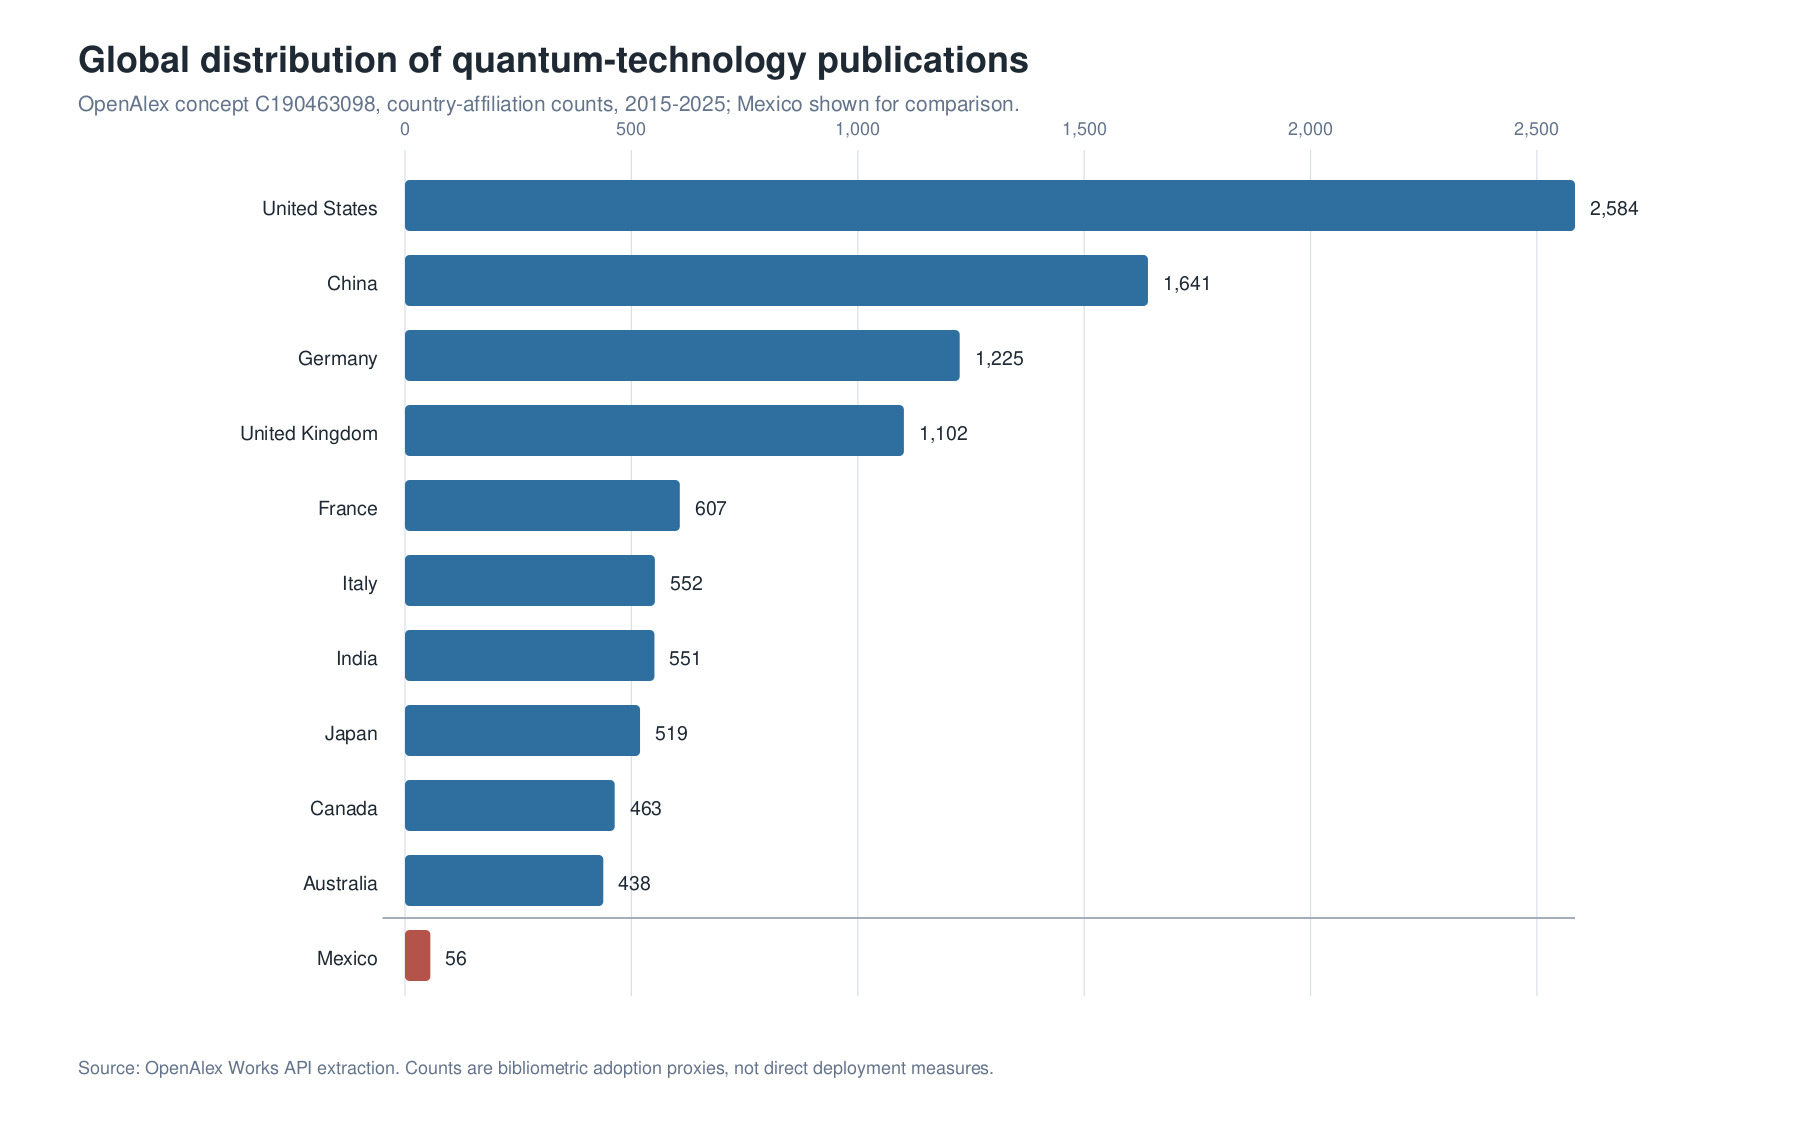
\includegraphics[width=0.95\textwidth,height=\textheight]{figures/fig1_global_country_distribution.png}
\caption{Global distribution of quantum-technology publication capacity.
OpenAlex country-affiliation counts for the concept ``Quantum
technology'' show the scale difference between leading research systems
and Mexico's measurable but smaller publication base.}
\end{figure}

\section{4. Results}\label{results}

\subsection{4.1 The International Readiness
Gap}\label{the-international-readiness-gap}

The international evidence indicates a substantial gap between expected
quantum impact and organizational preparation. OECD summarizes executive
surveys in which high shares of respondents expect quantum technologies
to affect their sectors, while far smaller shares report strategic
planning, budgets, or identified commercial use cases. In one UK
executive survey summarized by OECD, 97\% of respondents expected
disruption, yet only about one-third had begun strategic readiness
planning. In a financial-sector survey, 87\% saw quantum computing as an
opportunity, while 73\% lacked an identified application with real
commercial advantage and 87\% had no dedicated quantum budget. ISACA's
2025 survey reports that only 20\% of respondents had formal quantum
readiness plans despite broad expectations of future impact
(\citeproc{ref-oecd2026}{OECD 2026}).

For Mexico, the implication is that awareness-building is not
sufficient. Institutional readiness depends on cryptographic
inventories, procurement criteria, technical workforce programmes, pilot
funding, access to testing infrastructure, and mechanisms for comparing
quantum solutions against classical baselines.

\begin{figure}
\centering
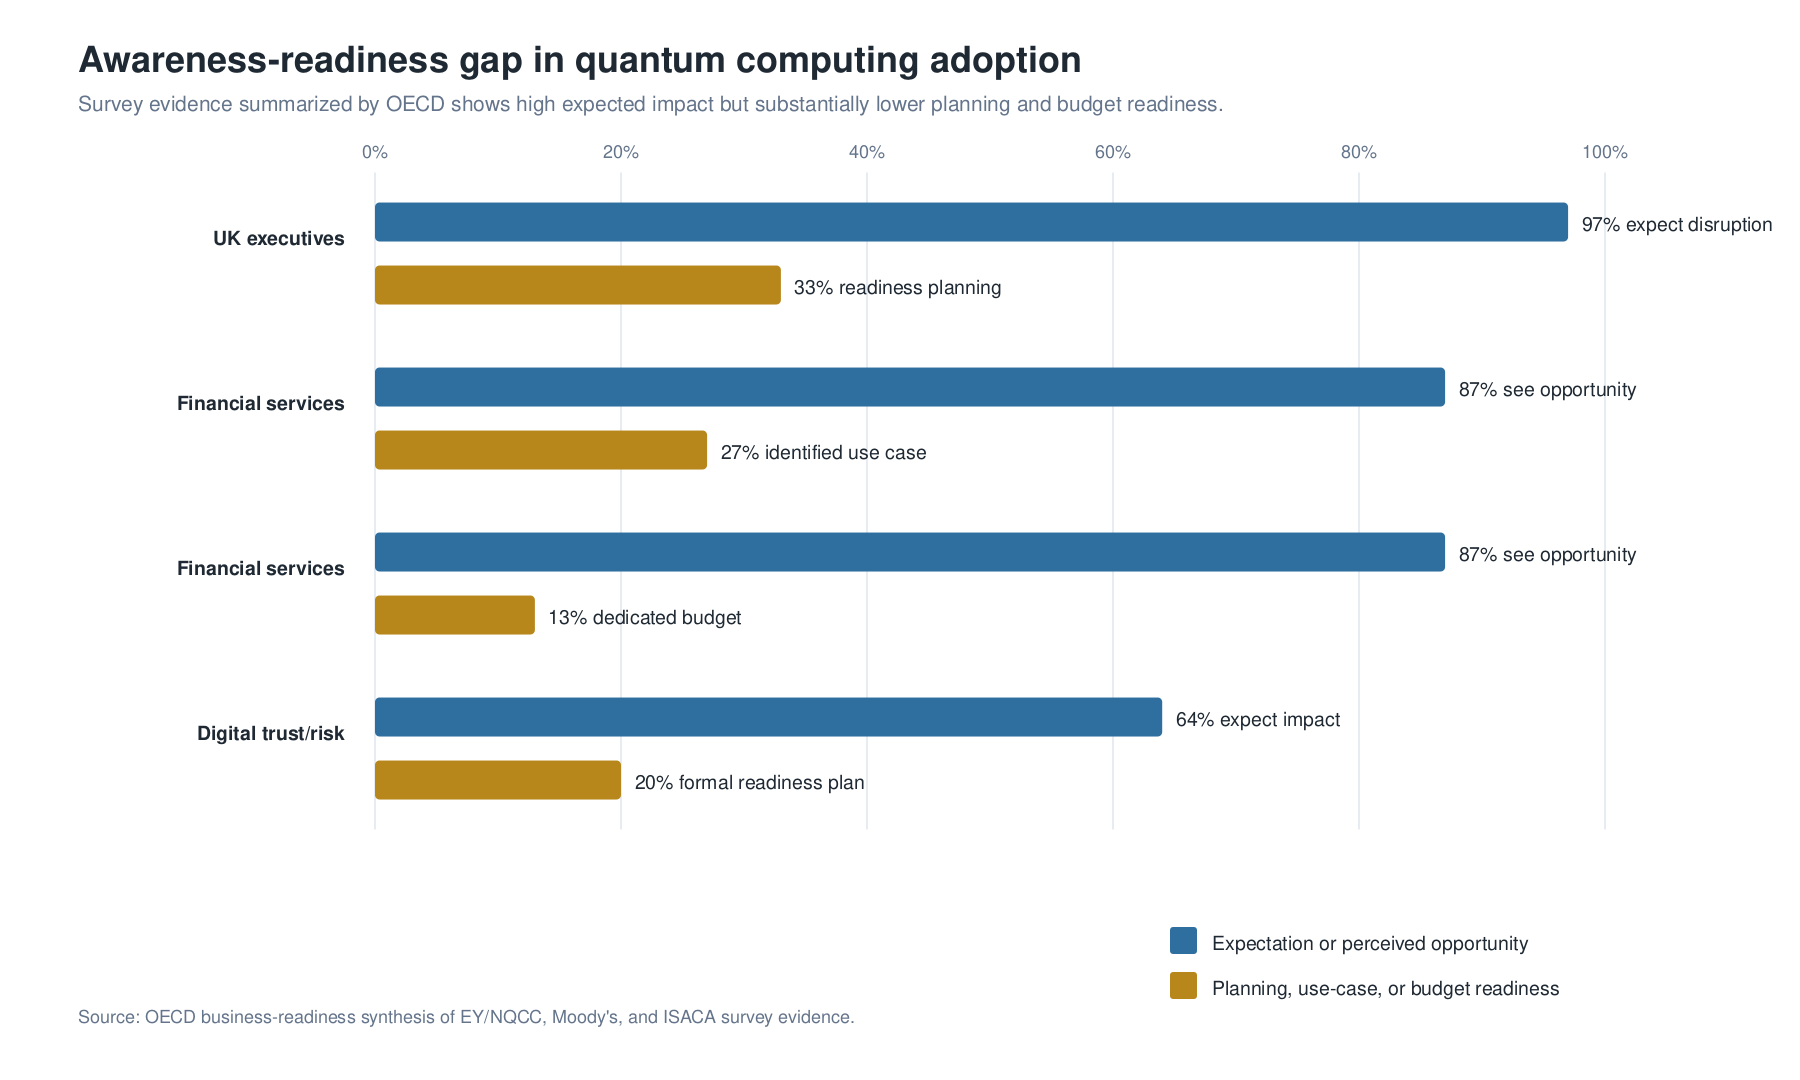
\includegraphics[width=0.95\textwidth,height=\textheight]{figures/fig3_readiness_gap.png}
\caption{Awareness-readiness gap in quantum computing adoption. Survey
evidence summarized by OECD indicates that high expected impact coexists
with substantially lower levels of planning, use-case definition, and
dedicated budget formation.}
\end{figure}

\subsection{4.2 Mexico's Research Absorptive
Capacity}\label{mexicos-research-absorptive-capacity}

OpenAlex bibliometric data indicate that Mexico has a small but
identifiable research base in quantum technology. In the 2015-2025 query
for the ``Quantum technology'' concept, Mexico appears with 56 works.
This is modest compared with the United States (2,584), China (1,641),
Germany (1,225), the United Kingdom (1,102), and France (607). Within
the Mexico-affiliated subset, the leading institutions are Universidad
Nacional Autonoma de Mexico (20 works), Instituto Politecnico Nacional
(13), and Tecnologico de Monterrey (10). These counts are not a ranking
of technological readiness, but they indicate that Mexico is not
starting from zero. A national programme could use this base to organize
training, testbeds, applied research, and international collaboration.

\begin{figure}
\centering
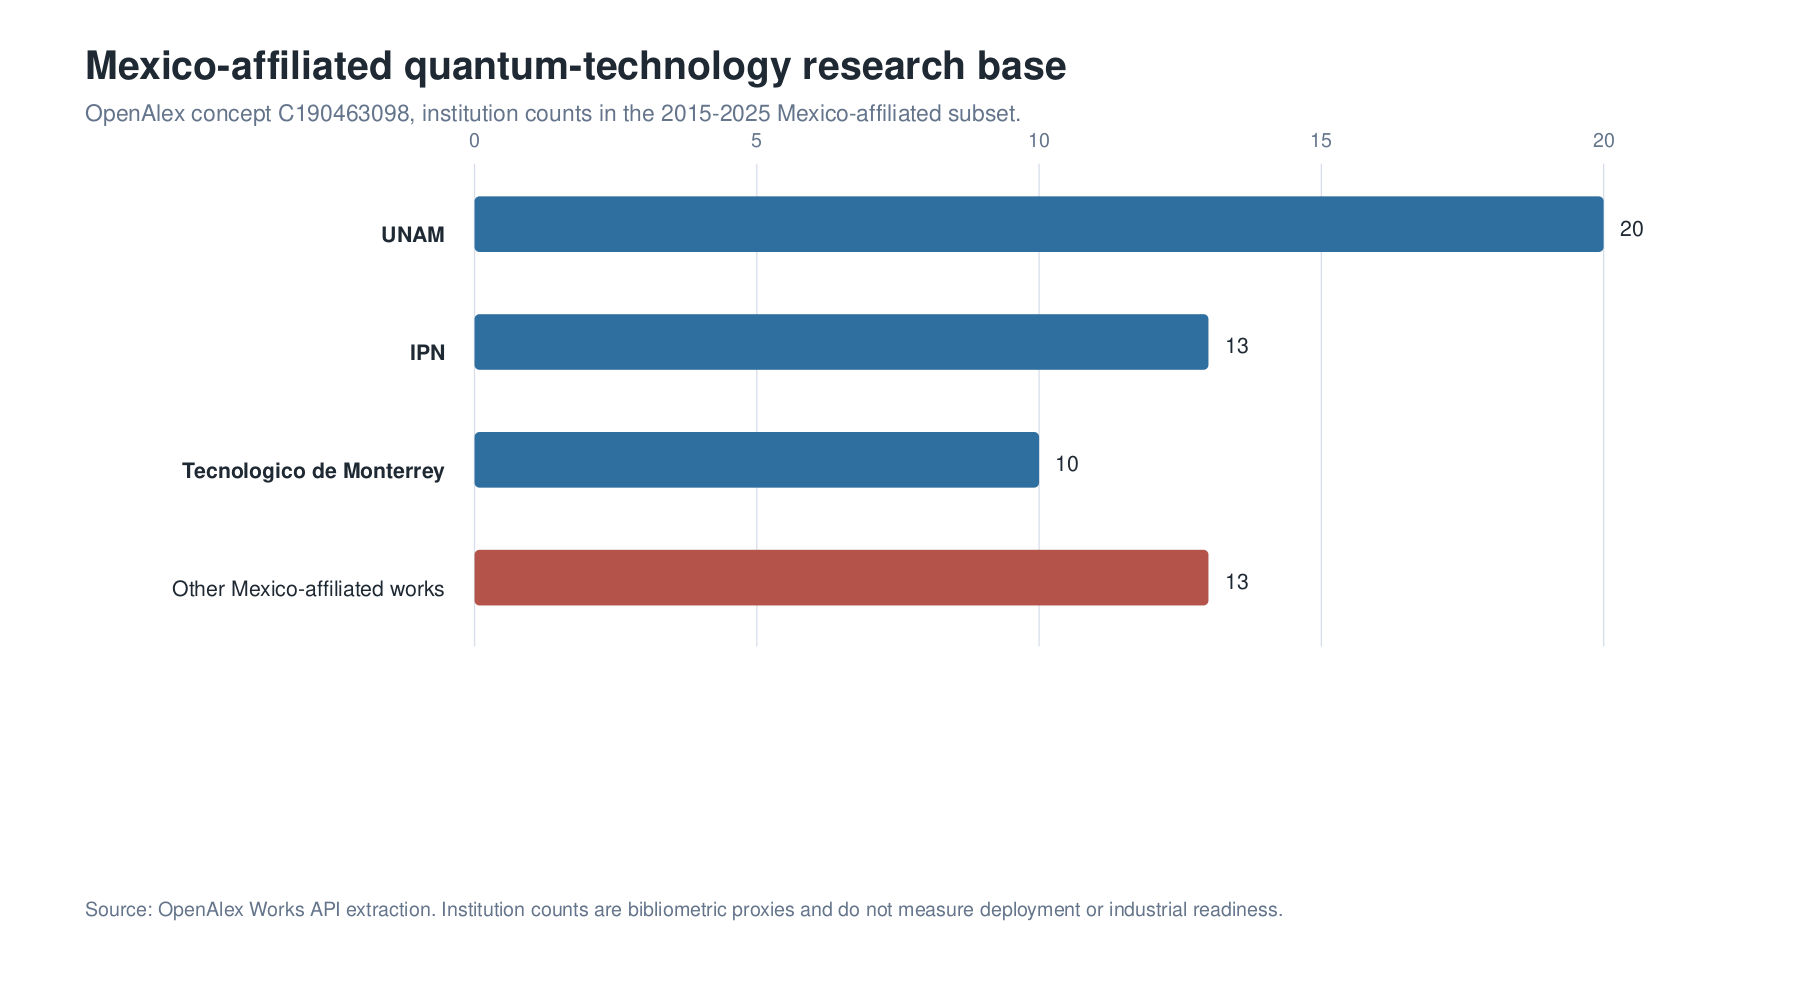
\includegraphics[width=0.92\textwidth,height=\textheight]{figures/fig6_mexico_institutions.png}
\caption{Mexico-affiliated quantum-technology research base. OpenAlex
institution counts identify UNAM, IPN, and Tecnologico de Monterrey as
leading affiliations in the extracted Mexico subset.}
\end{figure}

\subsection{4.3 Domain Priorities for Mexican Digital
Transformation}\label{domain-priorities-for-mexican-digital-transformation}

Four domains emerge as policy-relevant. First, post-quantum cryptography
is the clearest near-term priority because it addresses long-lived
cybersecurity risk and can be implemented through standards, software,
and protocol migration. Second, quantum sensing is the strongest early
application domain for Mexican public problems, including groundwater,
infrastructure monitoring, geodesy, health, mining, energy systems, and
environmental risk. Third, quantum computing is most credible in the
near term as cloud-based and HPC-mediated experimentation, benchmarking,
workflow integration, and workforce development rather than immediate
domestic hardware acquisition. Fourth, quantum communication is a
specialized strategic infrastructure domain, suitable for research,
telecom experimentation, and high-value security pilots rather than
broad substitution for existing cybersecurity.

\begin{figure}
\centering
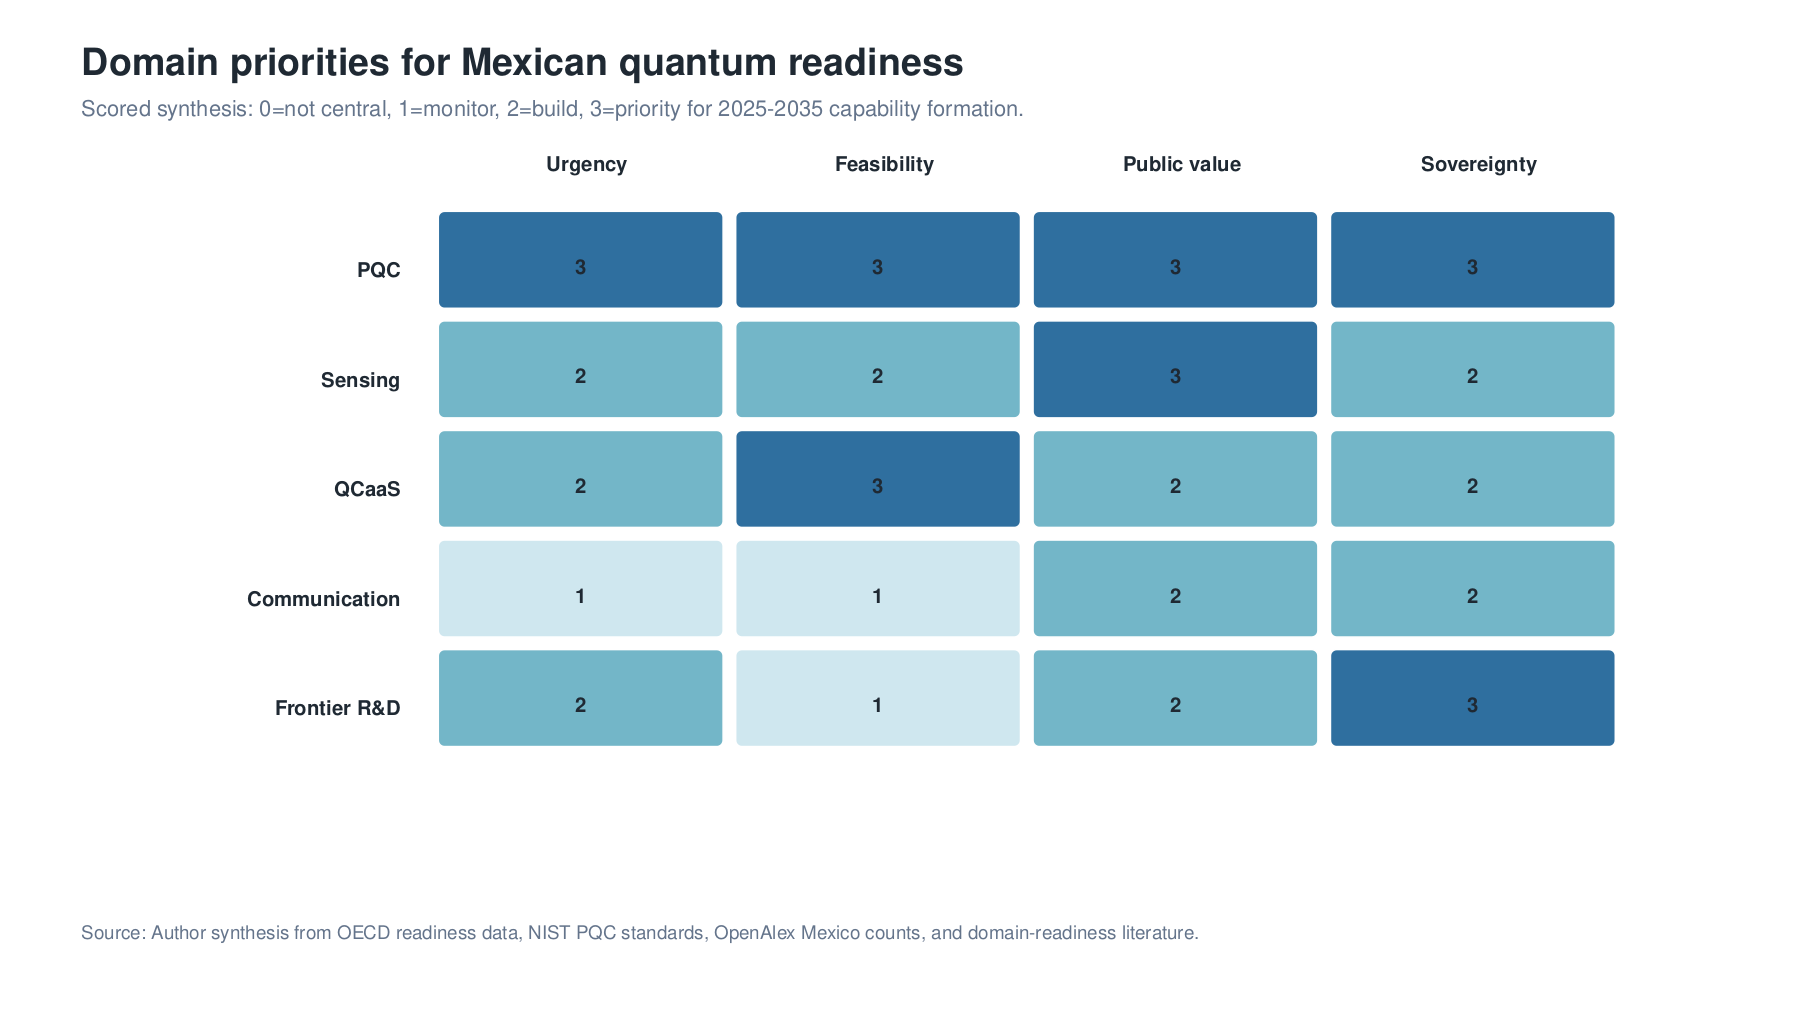
\includegraphics[width=0.95\textwidth,height=\textheight]{figures/fig7_mexico_domain_priority.png}
\caption{Domain priorities for Mexican quantum readiness. The scoring
matrix summarizes urgency, feasibility, public value, and sovereignty
relevance across PQC, sensing, QCaaS, quantum communication, and
frontier research.}
\end{figure}

\section{5. Discussion}\label{discussion}

The findings frame Mexico's quantum transition as a problem of
capability sequencing. The first stage is institutional preparation: PQC
migration planning, training, standards, and access to QCaaS and HPC-QC
platforms. The second stage is applied experimentation: sectoral sensing
pilots, quantum software testbeds, hybrid workflow pilots, and
procurement methods that require comparison with classical alternatives.
The third stage is strategic integration: participation in supply
chains, international research partnerships, and frontier research that
can produce long-term scientific autonomy.

HPC is central to this sequence because it gives quantum computing an
operational institutional home. Mexican universities, laboratories, and
public agencies do not need to wait for domestic ownership of
fault-tolerant quantum computers before building quantum capability.
They can begin by connecting quantum programming, quantum simulation,
and QCaaS access to existing scientific-computing environments. This
approach also disciplines adoption claims: quantum subroutines are
evaluated inside complete workflows, with queue latency, data movement,
error mitigation, classical optimization, and verification included in
the performance assessment.

This sequencing also changes how quantum technologies relate to
artificial intelligence, machine learning, and blockchain. Quantum
technologies are not replacements for these digital agendas; they alter
the infrastructure beneath them. AI can support quantum calibration,
sensor interpretation, and materials discovery. Distributed ledgers and
public records require post-quantum security if they are to preserve
long-lived trust. Cloud platforms become the initial channel through
which most Mexican institutions will access quantum processors.
Cybersecurity links the entire agenda because current public-key
cryptography will be affected by future quantum capability.

\section{6. Policy Implications}\label{policy-implications}

The analysis supports six policy implications. First, PQC migration is
best treated as a digital-infrastructure programme rather than as a
narrow cybersecurity procurement. Second, quantum sensing has the
strongest public-value fit when linked to concrete missions in water,
energy, health, civil protection, infrastructure, and environmental
monitoring. Third, a national QCaaS, HPC-QC, and quantum software
testbed would build human capital without premature hardware lock-in.
Fourth, procurement requires benchmarks, classical baselines,
interoperability, and total-cost analysis. Fifth, universities and
research centres can be connected through a national quantum workforce,
metrology, and scientific-computing network. Sixth, frontier research
funding is most strategic when it generates instrumentation capacity and
international scientific relevance.

\section{7. Conclusion}\label{conclusion}

Quantum technologies are relevant to Mexican digital transformation
because they affect the security, measurement, and computational layers
on which digital society depends. The evidence does not support a
passive wait-and-see posture. It also does not support symbolic
investment in immature hardware without institutional capacity. The most
defensible strategy is a sequenced one: PQC, sensing, workforce,
standards, and cloud-based plus HPC-mediated experimentation in the
first phase; applied testbeds in the second; and frontier research plus
international collaboration as the long-term basis for scientific
autonomy.

\section{Acknowledgments}\label{acknowledgments}

This manuscript was prepared for the Quantum Technologies track of the
twenty-third edition of the Global Information Technology Management
Association Annual Conference, Monterrey, Mexico, May 6-8, 2026. The
author acknowledges his role as Track Chair for Quantum Technologies and
gratefully acknowledges Rogelio Marín and the Centro de Investigación en
Matemáticas, A.C. for intellectual support and institutional context.
All interpretations and remaining errors are the author's
responsibility.

\section{Data Availability}\label{data-availability}

The quantitative evidence underlying the analysis comes from OECD public
reports, NIST/NSA/CISA guidance, and OpenAlex bibliometric queries.
Processed OpenAlex CSV extracts for country and year counts are
deposited in the companion research repository.

\section{Code Availability}\label{code-availability}

The companion research repository is available at
https://github.com/ekaropolus/quantum-technologies-national-strategy. It
contains the source manuscript, processed data, BibTeX bibliography,
figure-generation code, and reproducible build script used to generate
the manuscript outputs. The repository is intended to support inspection
of the OpenAlex extracts, regeneration of figures, and reconstruction of
the PDF, TeX, and DOCX versions from the manuscript sources.

\section{Limitations}\label{limitations}

The Mexico-specific analysis uses global adoption evidence and
bibliometric proxies rather than a dedicated national survey of Mexican
firms and agencies. A future empirical extension would require Mexican
stakeholder interviews, sector surveys, and cryptographic asset
inventory data.

\section{Competing Interests}\label{competing-interests}

The author declares no competing interests.

\section{References}\label{references}

\phantomsection\label{refs}
\begin{CSLReferences}{1}{0}
\bibitem[\citeproctext]{ref-beck2024}
Beck, Thomas, Alessandro Baroni, Ryan Bennink, Gilles Buchs, Eduardo
Antonio Coello Perez, Markus Eisenbach, Rafael Ferreira da Silva, et al.
2024. {``Integrating Quantum Computing Resources into Scientific HPC
Ecosystems.''} \emph{Future Generation Computer Systems}.
\url{https://doi.org/10.1016/j.future.2024.06.058}.

\bibitem[\citeproctext]{ref-bova2020}
Bova, Francesco, Avi Goldfarb, and Roger G. Melko. 2020. {``The Emerging
Commercial Landscape of Quantum Computing.''} \emph{Nature Reviews
Physics} 2: 596--98. \url{https://doi.org/10.1038/s42254-020-00247-5}.

\bibitem[\citeproctext]{ref-cisaNistNsa2022}
CISA, NIST, and NSA. 2022. {``Preparing Critical Infrastructure for
Post-Quantum Cryptography.''}
\url{https://www.cisa.gov/sites/default/files/2022-09/cisa_insight_post_quantum_cryptography_508.pdf}.

\bibitem[\citeproctext]{ref-cohen1990}
Cohen, Wesley M., and Daniel A. Levinthal. 1990. {``Absorptive Capacity:
A New Perspective on Learning and Innovation.''} \emph{Administrative
Science Quarterly} 35 (1): 128--52.
\url{https://doi.org/10.2307/2393553}.

\bibitem[\citeproctext]{ref-cranganore2024}
Cranganore, Sandeep Suresh, Vincenzo De Maio, Ivona Brandic, and Ewa
Deelman. 2024. {``Paving the Way to Hybrid Quantum-Classical Scientific
Workflows.''} \emph{Future Generation Computer Systems} 158: 346--66.
\url{https://doi.org/10.1016/j.future.2024.04.030}.

\bibitem[\citeproctext]{ref-iadb2025}
Inter-American Development Bank. 2025. {``Quantum Technologies: Digital
Transformation, Social Impact, and Cross-Sector Disruption.''}
\url{https://publications.iadb.org/publications/english/document/Quantum_Technologies_Digital_Transformation_Social_Impact_and_Crosssector_Disruption.pdf}.

\bibitem[\citeproctext]{ref-kaur2022}
Kaur, Maninder, and Alberto Venegas-Gomez. 2022. {``Defining the Quantum
Workforce Landscape: A Review of Global Quantum Education
Initiatives.''} \emph{Optical Engineering} 61 (8): 081806.
\url{https://doi.org/10.1117/1.OE.61.8.081806}.

\bibitem[\citeproctext]{ref-kwon2026}
Kwon, Ohbyung, Seongjun Kwon, Timothy Jung, and Saifeddin Alimamy. 2026.
{``Factors Influencing the Adoption Intent of Quantum Computing in
Enterprises: An Innovation Adoption Process Perspective.''}
\emph{International Journal of Information Management} 86: 102978.
\url{https://doi.org/10.1016/j.ijinfomgt.2025.102978}.

\bibitem[\citeproctext]{ref-liu2024}
Liu, Jie, Huan Ma, Honghui Shang, Zhenyu Li, and Jinlong Yang. 2024.
{``Quantum-Centric High Performance Computing for Quantum Chemistry.''}
\emph{Physical Chemistry Chemical Physics} 26: 15831--43.
\url{https://doi.org/10.1039/D4CP00436A}.

\bibitem[\citeproctext]{ref-lundvall1992}
Lundvall, Bengt-Ake, ed. 1992. \emph{National Systems of Innovation:
Toward a Theory of Innovation and Interactive Learning}. London: Pinter.

\bibitem[\citeproctext]{ref-nelson1993}
Nelson, Richard R., ed. 1993. \emph{National Innovation Systems: A
Comparative Analysis}. New York: Oxford University Press.

\bibitem[\citeproctext]{ref-nist2024}
NIST. 2024. {``NIST Releases First 3 Finalized Post-Quantum Encryption
Standards.''}
\url{https://www.nist.gov/news-events/news/2024/08/nist-releases-first-3-finalized-post-quantum-encryption-standards}.

\bibitem[\citeproctext]{ref-nsa2024}
NSA. 2024. {``Post-Quantum Cybersecurity Resources.''}
\url{https://www.nsa.gov/Cybersecurity/Post-Quantum-Cybersecurity-Resources/}.

\bibitem[\citeproctext]{ref-oecd2025a}
OECD. 2025. {``An Overview of National Strategies and Policies for
Quantum Technologies.''} OECD Digital Economy Papers.
\url{https://www.oecd.org/en/publications/an-overview-of-national-strategies-and-policies-for-quantum-technologies_5e55e7ab-en.html}.

\bibitem[\citeproctext]{ref-oecd2026}
---------. 2026. {``Building Business Readiness for Quantum
Computing.''} OECD Digital Economy Papers.
\url{https://www.oecd.org/en/publications/building-business-readiness-for-quantum-computing_ee847e5f-en.html}.

\bibitem[\citeproctext]{ref-openalex2026}
OpenAlex. 2026. {``OpenAlex Works API.''}
\url{https://docs.openalex.org/}.

\bibitem[\citeproctext]{ref-preskill2018}
Preskill, John. 2018. {``Quantum Computing in the NISQ Era and
Beyond.''} \emph{Quantum} 2: 79.
\url{https://doi.org/10.22331/q-2018-08-06-79}.

\bibitem[\citeproctext]{ref-qedc2022}
QED-C. 2022. {``Guide to Building a Quantum Technician Workforce.''}
\url{https://quantumconsortium.org/publication/guide-to-building-a-quantum-technician-workforce-2/}.

\end{CSLReferences}

\end{document}
